\documentclass{standalone}
\usepackage{tikz}

\begin{document}
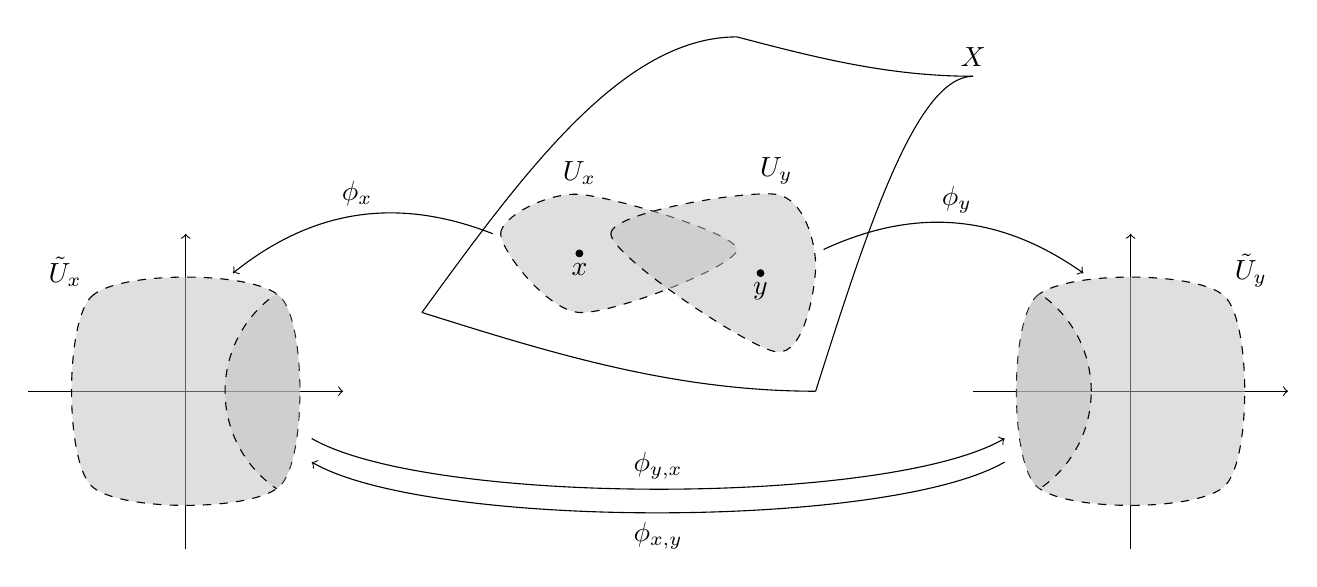
\begin{tikzpicture}
\draw (-2,0) node(a){};
\draw (3,-1) node(b){};
\draw (5,3) node(c){};
\draw (2,3.5) node(d){};

\draw (a) sin (b);
\draw (b) sin (c);
\draw (a) sin (d);
\draw (d) sin (c);

\draw (c) node[above]{$ X $};

\filldraw[dashed, fill=gray!50, fill opacity=0.5] plot[smooth cycle] coordinates{(0,0) (-1,1)
	(0,1.5) (2, 0.8)};
\filldraw[dashed, fill=gray!50, fill opacity=0.5] plot[smooth cycle] coordinates{(2.5,-0.5) (0.4,1)
	(2.5,1.5) (3, 0.6)};
\fill (0,0.75) circle (0.05) node[below]{$ x $};
\fill (2.3,0.5) circle (0.05) node[below]{$ y $};
\draw (0,1.5) node[above]{$ U_x $};
\draw (2.5,1.5) node[above]{$ U_y $};

\begin{scope}[xshift=7cm, yshift=-1cm]
\draw[->] (-2,0) -- (2,0);
\draw[->] (0,-2) -- (0,2);

\filldraw[dashed, fill=gray!50, fill opacity=0.5] plot[smooth cycle]
	coordinates{(-1.2, -1.2) (-1.2, 1.2) (1.2, 1.2) (1.2, -1.2)};
\begin{scope}
\clip plot[smooth cycle] coordinates{(-1.2, -1.2) (-1.2, 1.2) (1.2, 1.2) (1.2,
	-1.2)};
\filldraw[dashed, fill=gray!50, fill opacity=0.5] (-2,0) circle (1.5);
\end{scope}

\draw (1.2, 1.2) node[anchor=south west]{$ \tilde{U}_{y} $};
\end{scope}

\begin{scope}[xshift=-5cm, yshift=-1cm]
\draw[->] (-2,0) -- (2,0);
\draw[->] (0,-2) -- (0,2);

\filldraw[dashed, fill=gray!50, fill opacity=0.5] plot[smooth cycle]
	coordinates{(-1.2, -1.2) (-1.2, 1.2) (1.2, 1.2) (1.2, -1.2)};

\begin{scope}
\clip plot[smooth cycle] coordinates{(-1.2, -1.2) (-1.2, 1.2) (1.2, 1.2) (1.2,
	-1.2)};
\filldraw[dashed, fill=gray!50, fill opacity=0.5] (2,0) circle (1.5);
\end{scope}

\draw (-1.2, 1.2) node[anchor=south east]{$ \tilde{U}_{x} $};
\end{scope}

\draw[->, bend right] (-1.1,1) to node[above]{$ \phi_x $} ({0.6-5}, {1.5-1});
\draw[->, bend left] (3.1, 0.8) to node[above]{$ \phi_y $} ({-0.6+7}, {1.5-1});
\draw[->, bend right, looseness=0.5] ({1.6-5}, {-0.6-1}) to node[above]{$ \phi
	_{y,x} $} ({-1.6+7}, {-0.6-1});
\draw[<-, bend right, looseness=0.5] ({1.6-5}, {-0.9-1}) to node[below]{$ \phi
	_{x,y} $} ({-1.6+7}, {-0.9-1});

\end{tikzpicture}
\end{document}
